% MODELO DE RELATÓRIO DE FÍSICA EXPERIMENTAL I POR RODRIGO AMORIM
% BASEADO NO MODELO ORIGINAL (REVTEX 4-2)
\documentclass[aps,prb,12pt,onecolumn,amsmath,amssymb]{revtex4-2}
%----------------------------------
% PACOTES
%----------------------------------
\usepackage[brazil]{babel}
\usepackage[caption=false]{subfig}
\usepackage{graphicx}
\usepackage{bm}
\usepackage{microtype}
\usepackage{booktabs}
\usepackage{multirow}
\usepackage{siunitx}
\usepackage{ragged2e}
\usepackage{setspace}
\usepackage{hyperref}
%----------------------------------
% Configuração numérica
%----------------------------------
\sisetup{output-decimal-marker = {,}}
%----------------------------------
% Configuração das tabelas
%----------------------------------
\setlength{\tabcolsep}{12pt}       % espaçamento horizontal entre colunas
\renewcommand{\arraystretch}{1.15} % espaçamento vertical entre linhas
%----------------------------------
% Comandos matemáticos úteis
%----------------------------------
\newcommand{\med}[1]{\overline{#1}}                     % média aritmética
\newcommand{\avg}[1]{\left\langle #1 \right\rangle}     % valor esperado
\newcommand{\pd}[2]{\dfrac{\partial #1}{\partial #2}}   % derivadas parciais
%----------------------------------
% Configurações de idioma para legendas
%----------------------------------
\renewcommand{\tablename}{Tabela}
\renewcommand{\figurename}{Figura}
%----------------------------------
\begin{document}

\title{Relatório de Física Experimental I: Mecânica \\ \large Título do Experimento}

\author{Rodrigo Amorim, Rodrigo Alves, Rodrigo Montey e Rodrigo Silva}
\affiliation{Instituto Federal de Educação, Ciência e Tecnologia de Goiás, Campus Goiânia, GO, Brasil}

\begin{abstract}
O resumo deve apresentar, em um único parágrafo, o fenômeno investigado, o objetivo, o método empregado e o resultado mais importante, incluindo sua incerteza. Como orientação, considere: \textit{Neste trabalho, determinou-se experimentalmente a densidade de um sólido cilíndrico por meio de medições de massa, diâmetro e altura. O volume foi calculado a partir das dimensões geométricas e a incerteza da densidade foi obtida por propagação das incertezas das grandezas de entrada. O resultado, $\rho=(\ldots\pm\ldots)\,\mathrm{g/cm^3}$, foi comparado com valores de referência para discutir a possível composição do material.} Substitua as lacunas por resultados efetivamente obtidos; não antecipe conclusões não sustentadas pelos dados.
\end{abstract}

\maketitle

% =================================================
\section{Introdução}
% =================================================
A Introdução deve apresentar o fenômeno mecânico ou a propriedade física investigada e fornecer somente a fundamentação necessária à compreensão do experimento. O texto deve responder às seguintes questões:
\begin{itemize}
    \item Qual fenômeno ou propriedade física está sendo investigado?
    \item Qual é sua importância para a Mecânica?
    \item Qual modelo teórico ou modelo de medição será empregado?
    \item Quais grandezas serão medidas diretamente e quais serão determinadas indiretamente?
    \item Qual resultado poderá ser confrontado com um valor de referência ou com outra medição?
\end{itemize}
Não é necessário reproduzir toda a teoria apresentada em sala de aula ou na apostila. Por exemplo, na determinação da densidade de um cilindro homogêneo e regular, pode-se utilizar
\begin{align}
    \rho = \dfrac{m}{V} = \dfrac{4m}{\pi d^2 h},
\end{align}
em que $\rho$ é a densidade, $m$ é a massa, $V$ é o volume, $d$ é o diâmetro e $h$ é a altura do cilindro. O modelo pressupõe uma geometria aproximadamente cilíndrica e dimensões representativas do objeto.

Nos demais experimentos da disciplina, apresente a relação adequada, como $F = k\Delta x$ para o módulo da força elástica em uma mola ideal ou $g = 4\pi^2l/T^2$ para a determinação da aceleração da gravidade com um pêndulo simples na aproximação de pequenas oscilações. Todas as grandezas e hipóteses relevantes devem ser definidas. Ao final da Introdução, deve estar claro \textbf{o que será investigado e como o modelo relaciona as grandezas experimentais}.

% =================================================
\section{Objetivos}
% =================================================
Esta seção deve ser curta e direta. Indique o que se pretende determinar, verificar ou comparar. Para o experimento de densidade, por exemplo:
\begin{itemize}
    \item determinar a densidade de um cilindro a partir de medições de sua massa e dimensões;
    \item estimar as incertezas associadas às grandezas medidas diretamente;
    \item calcular a incerteza da densidade por propagação;
    \item comparar a densidade obtida com valores de referência, considerando as incertezas e as limitações do método.
\end{itemize}
Para os demais experimentos, substitua esses objetivos pelos correspondentes ao roteiro. Evite desenvolver a teoria ou antecipar resultados nesta seção.

% =================================================
\section{Materiais e Métodos}
% =================================================
Esta seção deve permitir que outra pessoa compreenda como o experimento foi realizado e, em princípio, possa reproduzi-lo. Descreva o procedimento realmente adotado, não apenas aquele previsto no roteiro.

% -------------------------------------------------
\subsection{Materiais utilizados}
% -------------------------------------------------
Identifique os equipamentos e objetos utilizados. Para o exemplo de densidade de sólidos regulares, a lista poderia conter:
\begin{itemize}
    \item cilindro metálico ou outro sólido regular investigado;
    \item balança digital, com identificação do modelo e da resolução;
    \item paquímetro, com identificação do modelo e da resolução;
    \item outros instrumentos efetivamente empregados, se houver.
\end{itemize}
Informe, sempre que disponíveis, a \textbf{marca, o modelo, a resolução e eventuais informações de calibração} dos instrumentos. Não atribua ao equipamento uma incerteza sem justificar o critério de avaliação utilizado.

% -------------------------------------------------
\subsection{Montagem e procedimento experimental}
% -------------------------------------------------
Descreva como o objeto foi posicionado e como cada grandeza foi medida. No exemplo, explique como se determinou a massa com a balança e em quais posições foram feitas as leituras de diâmetro e altura com o paquímetro. Informe a quantidade de leituras, se houve repetição das medições e como foram obtidos os valores representativos. Evite narrativas cronológicas sem importância para a reprodutibilidade. A montagem ou o objeto investigado pode ser ilustrado por uma fotografia ou esquema.
\begin{figure}[ht]
    \centering
    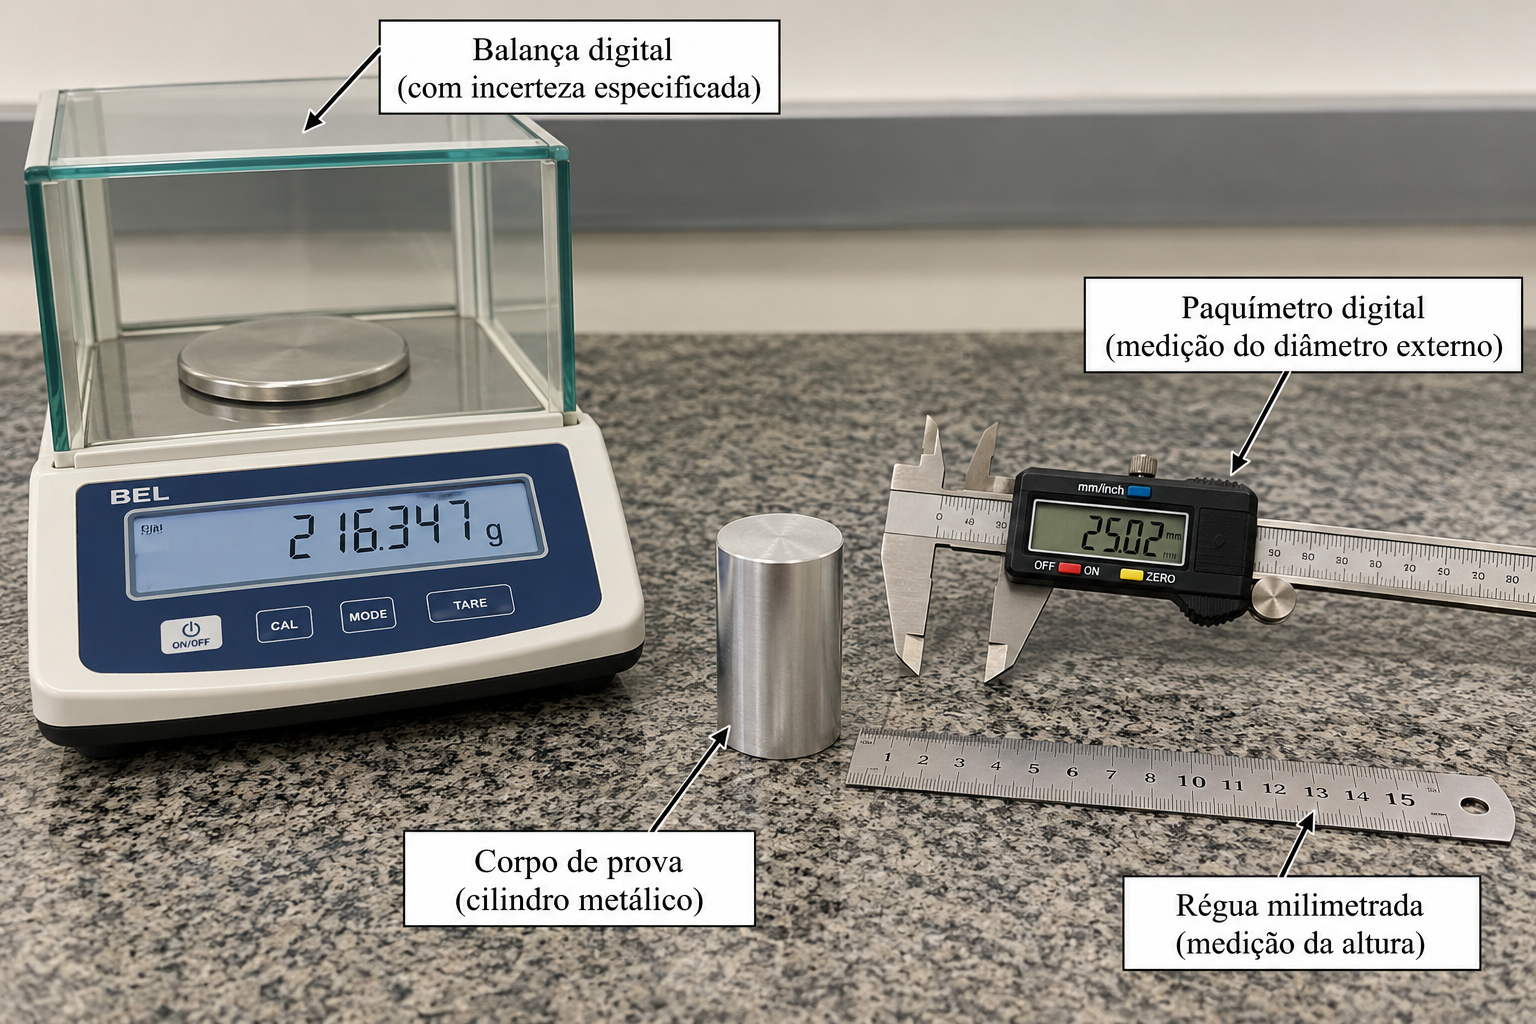
\includegraphics[width=0.60\textwidth]{montagem_experimental.png}
    \caption{Montagem experimental utilizada para a realização das medidas.}
    \label{fig:montagem}
\end{figure}

No texto, esclareça:
\begin{itemize}
    \item quais dimensões ou variáveis foram medidas diretamente;
    \item qual instrumento foi empregado em cada medição;
    \item quais resoluções e condições de leitura foram consideradas;
    \item quantas medições foram efetuadas e se foram realizadas em posições diferentes;
    \item como foram identificadas e consideradas eventuais fontes de variabilidade.
\end{itemize}

% -------------------------------------------------
\subsection{Modelo teórico}
% -------------------------------------------------
Apresente o modelo de medição e o tratamento aplicado aos dados. Na determinação da densidade de um cilindro,
\begin{align}
    \rho = \dfrac{4m}{\pi d^2 h}.
\end{align}
De maneira geral, uma grandeza obtida indiretamente pode ser escrita como
\begin{align}
    y = y(x_1,x_2,\ldots,x_n),
\end{align}
em que $x_1,x_2,\ldots,x_n$ são as grandezas de entrada. Apresente cada resultado experimental acompanhado de sua incerteza, por exemplo,
\begin{align}
    x = \left(\overline{x} \pm u_x\right)\,\text{unidade}.
\end{align}

As incertezas devem ser avaliadas de acordo com a natureza das informações disponíveis. A \textbf{avaliação do Tipo A} utiliza a distribuição estatística de medições repetidas; a \textbf{avaliação do Tipo B} emprega informações como resolução, certificado de calibração e especificações instrumentais. Na terminologia da disciplina, a \textbf{avaliação do Tipo C} corresponde à propagação de incertezas em grandezas determinadas indiretamente. Essas designações se referem a procedimentos de avaliação, não a três espécies distintas de erro.

Para uma grandeza indireta $y = y(x_1,x_2,\ldots,x_n)$, considerando incertezas padrão de entrada não correlacionadas e a aproximação linear,
\begin{align}
    u_y = \sqrt{\left(\dfrac{\partial y}{\partial x_1}u_{x_1}\right)^2 + \left(\dfrac{\partial y}{\partial x_2}u_{x_2}\right)^2 + \cdots +
    \left(\dfrac{\partial y}{\partial x_n}u_{x_n}\right)^2}.
\end{align}
Para o cilindro, supondo $m$, $d$ e $h$ não correlacionados, obtém-se
\begin{align}
    u_\rho = \rho\sqrt{\left(\dfrac{u_m}{m}\right)^2 + \left(2\dfrac{u_d}{d}\right)^2 + \left(\dfrac{u_h}{h}\right)^2}.
\end{align}
Assim, o resultado deve ser apresentado na forma
\begin{align}
    \rho = (\overline{\rho}\pm u_\rho)\,\mathrm{g/cm^3},
\end{align}
com valores e arredondamentos consistentes. A notação $\overline{\rho}$ representa aqui o valor principal reportado e não implica, necessariamente, a média aritmética de densidades distintas.

% =================================================
\section{Resultados e Discussão}
% =================================================
Apresente os resultados obtidos e discuta seu significado físico. Organize os valores em \textbf{tabelas e, quando pertinentes ao roteiro, gráficos}. Inclua valores principais, incertezas, unidades e informações suficientes para interpretar o procedimento. Os números das tabelas a seguir são \textbf{exclusivamente ilustrativos}, não resultados reais de uma aula.

% -------------------------------------------------
\subsection{Dados experimentais}
% -------------------------------------------------
A tabela principal deve apresentar as grandezas medidas acompanhadas das incertezas reportadas. No exemplo, considere três cilindros semelhantes, cujas massas e dimensões foram determinadas diretamente:
\begin{table}[ht]
    \centering
    \begin{tabular}{cccc}
        \toprule
        Corpo & $m$ (g) & $d$ (mm) & $h$ (mm) \\
        \midrule
        1 & 33,90 $\pm$ 0,01 & 20,00 $\pm$ 0,02 & 40,00 $\pm$ 0,05 \\
        2 & 34,02 $\pm$ 0,01 & 20,04 $\pm$ 0,02 & 40,02 $\pm$ 0,05 \\
        3 & 33,85 $\pm$ 0,01 & 19,98 $\pm$ 0,02 & 39,98 $\pm$ 0,05 \\
        \bottomrule
    \end{tabular}
    \caption{Dados ilustrativos de massa, diâmetro e altura de três corpos cilíndricos, com as respectivas incertezas padrão adotadas para exemplificar o tratamento de dados.}
    \label{tab:dados}
\end{table}

No relatório real, esclareça se os resultados representam leituras únicas, médias de medições repetidas ou valores obtidos a partir de posições distintas do corpo. Justifique as incertezas indicadas; \textbf{não reproduza os valores ilustrativos como se fossem especificações dos equipamentos}.

% -------------------------------------------------
\subsection{Cálculo das incertezas instrumentais}
% -------------------------------------------------
Informe as informações metrológicas efetivamente utilizadas na avaliação do Tipo B, tais como a resolução, a documentação do fabricante, certificados de calibração e a distribuição atribuída. A tabela abaixo é apenas um exemplo de organização:
\begin{table}[ht]
    \centering
    \begin{tabular}{cccc}
        \toprule
        Grandeza & Instrumento & Resolução & Critério de avaliação \\
        \midrule
        $m$ & Balança digital & 0,01 g & Consultar especificação/calibração \\
        $d$ e $h$ & Paquímetro & 0,01 mm & Consultar especificação/calibração \\
        \bottomrule
    \end{tabular}
    \caption{Exemplo de registro de instrumentos e resoluções. Os valores não constituem especificações de um modelo particular nem determinam, por si, as incertezas da Tabela~\ref{tab:dados}.}
    \label{tab:incertezas}
\end{table}

Se forem utilizados resultados de medições repetidas, explicite também o cálculo da contribuição do Tipo A. Se houver mais de uma contribuição independente para a mesma grandeza, informe como foram combinadas. Não confunda \textbf{erro de medição}, \textbf{resolução} e \textbf{incerteza de medição}.

% -------------------------------------------------
\subsection{Grandezas calculadas}
% -------------------------------------------------
Apresente os valores determinados indiretamente, com as incertezas propagadas. No exemplo, para o corpo 1, usando $m = \num{33,90}$ g, $d = \num{20,00}$ mm e $h = \num{40,00}$ mm, tem-se
\begin{align}
    \rho_1 &= \dfrac{4m}{\pi d^2h} \simeq \SI{2,6977}{\gram\per\centi\meter\cubed}, \\
    u_{\rho_1} &= \rho_1\sqrt{\left(\dfrac{0,01}{33,90}\right)^2 + \left(2\frac{0,02}{20,00}\right)^2 + \left(\dfrac{0,05}{40,00}\right)^2}
    \simeq \SI{0,0064}{\gram\per\centi\meter\cubed}.
\end{align}
Os resultados devem ser arredondados de modo coerente com a incerteza, como ilustrado abaixo:
\begin{table}[ht]
    \centering
    \begin{tabular}{cc}
        \toprule
        Corpo & $\rho$ ($\mathrm{g/cm^3}$) \\
        \midrule
        1 & 2,6977 $\pm$ 0,0064 \\
        2 & 2,6951 $\pm$ 0,0064 \\
        3 & 2,7004 $\pm$ 0,0064 \\
        \bottomrule
    \end{tabular}
    \caption{Densidades ilustrativas obtidas a partir dos dados da Tabela~\ref{tab:dados}, com incertezas padrão propagadas, arredondadas a dois algarismos significativos.}
    \label{tab:resultados}
\end{table}

A discussão deve interpretar os dados à luz do modelo e das respectivas incertezas. Conforme o experimento, procure responder:
\begin{itemize}
    \item Os resultados são compatíveis entre si ou com os valores de referência adotados?
    \item Qual grandeza de entrada contribuiu mais para a incerteza final?
    \item As hipóteses do modelo são adequadas à montagem (por exemplo, geometria cilíndrica e homogeneidade)?
    \item Foram identificados efeitos como irregularidade geométrica, desalinhamento ou erro de zero?
    \item O procedimento permite sustentar as conclusões propostas?
\end{itemize}

Evite concluir que dois resultados concordam apenas porque seus valores numéricos são próximos. Uma comparação deve considerar suas incertezas e, quando solicitado na apostila ou pelo professor, aplicar um \textbf{teste de compatibilidade}. No experimento de densidade, uma tabela pode confrontar o resultado com uma referência bibliográfica:
\begin{table}[ht]
    \centering
    \begin{tabular}{ccc}
        \toprule
        Grandeza & Valor de referência & Valor experimental \\
        \midrule
        $\rho$ & $\rho_{\mathrm{ref}}$ (informar fonte e condições) & $(\overline{\rho}\pm u_\rho)$ \\
        \bottomrule
    \end{tabular}
    \caption{Modelo de comparação com um valor de referência. Substitua símbolos pelos resultados reais e informe a origem e a incerteza da referência, se disponível.}
    \label{tab:comparacao}
\end{table}

Nos experimentos de Mecânica que envolvam relações funcionais (por exemplo, força e deformação na lei de Hooke, período e comprimento no pêndulo simples), apresente os gráficos e ajustes solicitados no roteiro, incluindo os parâmetros ajustados e suas incertezas. Não acrescente gráficos sem finalidade na análise.

% =================================================
\section{Considerações Finais}
% =================================================
Retome os objetivos e apresente brevemente os resultados principais, sempre que possível com os respectivos valores e incertezas. Indique:
\begin{itemize}
    \item qual propriedade ou fenômeno mecânico foi investigado;
    \item qual grandeza foi determinada e com qual incerteza;
    \item se os resultados foram compatíveis com referências ou com outros procedimentos, segundo o critério adotado;
    \item quais hipóteses e limitações da montagem mais influenciaram a análise;
    \item qual aperfeiçoamento experimental seria relevante, se pertinente.
\end{itemize}
Não introduza resultados novos e não afirme que o experimento ``comprovou'' uma lei física. A conclusão deve refletir a evidência obtida, suas incertezas e o alcance do modelo utilizado.

% =================================================
\begin{thebibliography}{10}
% =================================================

\bibitem{taylor}
TAYLOR, J. R. \textit{Introdução à análise de erros: o estudo de incertezas em medições físicas}. Porto Alegre: Bookman, 2012.

\bibitem{vuolo}
VUOLO, J. H. \textit{Introdução à teoria de erros}. São Paulo: Blücher, 1996.

\bibitem{halliday}
HALLIDAY, D.; RESNICK, R.; WALKER, J. \textit{Fundamentos de Física}. 10. ed. Rio de Janeiro: LTC, 2016.

\bibitem{nussenzveig}
NUSSENZVEIG, H. M. \textit{Curso de Física Básica}. São Paulo: Edgard Blücher, 2002.

\bibitem{tipler}
TIPLER, P. A.; MOSCA, G. \textit{Física para Cientistas e Engenheiros}. Rio de Janeiro: LTC, 2006.

\bibitem{serway}
SERWAY, R. A.; JEWETT, J. W. \textit{Princípios de Física}. São Paulo: Cengage Learning, 2014.

\bibitem{young}
YOUNG, H. D.; FREEDMAN, R. A. \textit{Física Universitária}. São Paulo: Pearson, 2015.

\end{thebibliography}

\end{document}
